\documentclass[11pt,a4paper]{article}
\usepackage[T1]{fontenc}\usepackage[utf8]{inputenc}
\usepackage{lmodern,microtype,amsmath,amssymb,amsthm,mathtools}
\usepackage{booktabs,longtable,array,enumitem,xcolor,geometry,fancyhdr,hyperref,graphicx}
\geometry{margin=22mm}
\hypersetup{colorlinks=true,linkcolor=blue!55!black,urlcolor=blue,citecolor=blue!55!black,
 pdftitle={FIN ST1902--ST1991: Automorphism-Natural Cell-Complex No-Go, Refinement Conflict and the Hodge-Energy Frontier},
 pdfauthor={Krzysztof Żuchowski}}
\pagestyle{fancy}\fancyhf{}\fancyhead[L]{FIN ST1902--ST1991}\fancyhead[R]{Release 11.05}\fancyfoot[C]{\thepage}\setlength{\headheight}{14pt}
\newtheorem{theorem}{Theorem}\newcommand{\status}[1]{\textsf{[#1]}}

\begin{document}
\begin{titlepage}\centering\vspace*{14mm}
{\Huge\bfseries FIN ST1902--ST1991\par}\vspace{4mm}
{\LARGE Automorphism-Natural Cell-Complex No-Go,\par}\vspace{2mm}
{\LARGE Refinement Conflict and the Hodge-Energy Frontier\par}\vspace{12mm}
{\Large Krzysztof \.Zuchowski\par}
{\normalsize Independent Researcher --- Fractal Information Theory Project\par}
{\normalsize ORCID: 0009-0002-0909-3613\par}\vspace{9mm}
{\large Six adaptive research rounds --- 90 programmes\par}
{\large Release 11.05 --- 1 September 2026\par}
\vfill
\begin{minipage}{.87\textwidth}\small
This report tests the decisive target selected in Release 11.04: whether strict
FIN weights and exact refinement uniquely generate an automorphism-natural
oriented weighted 2-complex and gauge kinetic action.  The result is a strong
nonuniqueness theorem for support-only constructions and a conditional positive
product-cell construction relative to the refinement map.
\end{minipage}\vfill
{\small English mathematical and critical research report.}
\end{titlepage}

\begin{abstract}
ST1902--ST1991 analyse all automorphism-natural triangle face sets on the strict
weighted support, classify natural face measures, test exact $12\to24$
refinement, and falsify the most canonical flag/Hodge repair.

The weighted strict graph has automorphism group exactly $D_{12}$: its unique
maximum-weight distance-one edges form $C_{12}$, whose automorphisms are
dihedral, and those preserve every cyclic distance class.  The 220 triangles
split into 12 $D_{12}$ orbits of sizes
\[
12,24,24,24,24,12,24,24,12,12,24,4.
\]
Therefore automorphism-natural face sets are arbitrary unions of these orbits,
giving $2^{12}=4096$ possibilities.  Exact bit elimination proves that at
least 2542 have full rank 55 over $\mathbb F_2$ and hence kill first homology
over the rationals.  At least 338 are inclusion-minimal, all using five orbits.
Two different five-orbit complexes with 76 faces are independently verified by
exact rational rank to have rank 55.  Thus naturality, $H^1=0$, minimal orbit
count and equal minimum face count do not select a complex.

Face measures remain nonunique after a face set is fixed.  Positive
$D_{12}$-natural weights form an $(\mathbb R_+)^{12}$ orbit cone, or
$(\mathbb R_+)^5$ on a five-orbit minimal complex.  Five explicit positive
edge-derived rules---product, geometric mean, arithmetic mean, minimum and
maximum---span rank five across the triangle orbits and are not proportional.
Homogeneity does not remove the ambiguity: four of these rules have degree
one.  A discrete Hodge star and Wilson spectrum therefore depend on an
unsourced face inner product and overall gauge coupling.

Refinement supplies a conditional cellular repair but sharpens the no-go.  The
support of $A_{24}=A_{12}\otimes I_2+I_{12}\otimes B_q$ has 144 edges and
cycle rank 121.  Its flag complex contains 440 triangles with boundary rank
110, leaving
\[
\dim H^1=11.
\]
The typed product refinement supplies 66 edge-times-interval squares.  Their
addition raises the boundary rank to 121 and restores $H^1=0$.  These squares
are not cliques of the refined support.  Hence the support-only flag functor is
not product-refinement functorial; the product repair requires refinement
history and retains six square-orbit weights plus all inherited base choices.

Positive Wilson actions exist for every positive face measure, but neither
face areas nor action scale is sourced.  A finite heat trace has spectral
dimension zero at both asymptotic time extremes.  Under iterated binary
refinement,
\[
Z_k(t)=Z_{12}(t)\prod_{\ell=1}^k(1+e^{-2q_\ell t}),
\]
so every intermediate spectral-dimension profile depends explicitly on the
free sequence $q_\ell$.  A four-dimensional plateau can be fitted but is not
derived.  Complete-support nonlocal edges remain at every level, and the
actions are Euclidean rather than Lorentzian.

The full clique complex is a canonical support-only object, but it is the
11-simplex with 4096 simplices.  Its flag construction does not preserve the
exact product refinement; the product Hodge repair is not support-only and
still needs inner-product weights, cutoff scale and representations.

The decisive next theorem is therefore narrower and stronger than ``find a
2-complex'': classify all positive face inner products for which gauge
curvature energy commutes with FIN coarse/refinement maps over
$12\to24\to48$, and determine whether they are unique up to one overall
scale.  Failure would be a direct no-go for strict gauge geometry without new
assumptions.
\end{abstract}

\tableofcontents\newpage

\section{Round I: ST1902--ST1916 --- automorphisms and face sets}

The six strict weights are distinct and the distance-one weight is uniquely
maximal.  Any weighted-graph automorphism must preserve the distance-one
$C_{12}$ subgraph, so it lies in $D_{12}$.  Conversely every dihedral symmetry
preserves cyclic distance and all weights.  Therefore
\[
\operatorname{Aut}(A)=D_{12},\qquad|D_{12}|=24.
\]

The triangle orbits are characterized by cyclic side-distance triples.  There
are exactly twelve.  A face set is automorphism-natural precisely when it is a
union of complete orbits, yielding 4096 choices including the empty set and
the full triangle set.

To test whether topology/minimality removes the ambiguity, every orbit subset
was audited over $\mathbb F_2$ using exact bit Gaussian elimination.  At least
2542 subsets have triangle-boundary rank 55.  Because 55 is the maximum cycle
rank, each also has full rational rank.  At least 338 are inclusion-minimal,
all using five triangle orbits and between 76 and 120 faces.

Two explicit examples use orbit sets
\[
\{0,1,4,5,11\},qquad \{0,2,4,5,11\}.
\]
Each has 76 faces and exact rational boundary rank 55, yet they are distinct.

\begin{theorem}[automorphism/topology face-set no-go]
Weighted-graph naturality, vanishing $H^1$, inclusion minimality, five-orbit
support and minimum face count do not determine a unique strict 2-complex.
\end{theorem}

The census count is a rigorous lower bound for rationally full-rank complexes:
additional subsets could fail mod 2 while pass over the rationals.  This only
strengthens nonuniqueness.

\section{Round II: ST1917--ST1931 --- face measures}

On all triangles, a positive $D_{12}$-natural measure is constant on each orbit:
\[
\kappa\in(\mathbb R_+)^{12}.
\]
A selected five-orbit minimal complex retains $(\mathbb R_+)^5$.

For a triangle with edge weights $(w_1,w_2,w_3)$, the following are all
positive, symmetric and automorphism-natural:
\[
w_1w_2w_3,\quad(w_1w_2w_3)^{1/3},\quad
\frac{w_1+w_2+w_3}{3},\quad\min_iw_i,\quad\max_iw_i.
\]
Their twelve orbit-value vectors have numerical rank five.  The product and
geometric-mean vectors are not proportional; their ratio varies by orbit.
Geometric/arithmetic mean, minimum and maximum all scale linearly under
$w\mapsto cw$, so degree-one homogeneity still leaves at least four candidates.
More generally, arbitrary positive symmetric functions of two independent edge
ratios preserve degree-one naturality.

The face measure defines the 2-form inner product/Hodge star and changes the
gauge spectrum and EOM.  Even after relative weights are fixed, an overall
Wilson/gauge coupling remains free.  Dimensionless edge weights do not provide
face area, length squared or an action unit.

Maximum entropy requires a reference measure and constraints; a scalar Shannon
or moment datum cannot select a vector in a 12-dimensional cone.

\begin{theorem}[natural face-measure no-go]
Current strict edge weights plus positivity, symmetry and homogeneity do not
determine a unique face measure or gauge kinetic normalization.
\end{theorem}

\section{Round III: ST1932--ST1946 --- refinement conflict}

For generic $q>0$, the refined support is $K_{12}\square K_2$ with
\[
V=24,qquad E=144,qquad b_1=121.
\]
All 440 triangles lie entirely inside the two $K_{12}$ layers.  Exact mod-2
elimination gives triangle-boundary rank 110, so the flag complex has
\[
\dim H^1=121-110=11.
\]

The typed Cartesian product supplies one square for each of the 66 base edges:
\[
(i,0)\to(j,0)\to(j,1)\to(i,1)\to(i,0).
\]
The square boundaries have rank 66, but add exactly 11 directions modulo the
triangles.  Together, triangles and squares have rank 121 and kill $H^1$.

\begin{theorem}[flag/refinement conflict]
The support-only flag complex does not preserve first-homology closure under the
exact FIN product refinement.  Restoring closure requires non-clique square
cells obtained from the typed refinement map.
\end{theorem}

Every natural base face set still lifts to both layers, so refinement does not
choose among base candidates.  The 66 squares split into six cyclic-distance
orbits and retain a positive six-parameter weight cone.  If $q$ coincides with
a base edge weight, fiber edges cannot even be identified by weight alone;
refinement metadata is essential.

Thus a relative product-cell functor exists once the base complex and
refinement morphism are provided.  No absolute support-only functor is selected.

\section{Round IV: ST1947--ST1961 --- Wilson action and continuum}

For positive face coefficients,
\[
S_W=\sum_f\kappa_f(1-\operatorname{Re}U_f)\ge0.
\]
For small $U_f=e^{iF_f}$,
\[
1-\cos F_f=\frac12F_f^2+O(F_f^4),
\]
so every chosen positive measure supplies a consistent Euclidean quadratic
curvature action.  It does not fix face areas, lattice spacing, overall gauge
coupling or action units.

For the finite base spectrum,
\[
Z_{12}(t)=\sum_j e^{-t\lambda_j}
\]
tends to 12 as $t\to0$ and to 1 as $t\to\infty$.  Its logarithmic spectral
dimension tends to zero at both extremes; no finite graph has an asymptotic
continuum power law.

Iterated binary refinements give the exact factorization
\[
Z_k(t)=Z_{12}(t)\prod_{\ell=1}^k(1+e^{-2q_\ell t}),
\]
and
\[
d_s(t)=2t\left[
\frac{\sum_j\lambda_je^{-t\lambda_j}}{Z_{12}(t)}
+\sum_\ell\frac{2q_\ell}{e^{2q_\ell t}+1}
\right].
\]
The effective dimension depends on the entire free sequence $q_\ell$.  With
constant $q$, it grows with layer count at fixed intermediate time.  Geometric
or other sequences can shape plateaux, including a fitted value near four, but
that is a scaling assumption rather than a derivation.

Every refined vertex retains eleven complete-base neighbours.  Product
refinement adds fiber locality without removing base nonlocality.  The action
is Euclidean; Lorentzian signature and a causal cone remain absent.

\section{Round V: ST1962--ST1976 --- Hodge repair}

The full flag complex of base $K_{12}$ is canonical from support and equals the
11-simplex.  It has $H^1=0$ and 4096 simplices including the empty simplex.
This is mathematically canonical but not a 3+1-dimensional geometry.

At the refined level the flag complex contains triangles but not product
squares, producing eleven one-form Hodge zero modes.  The product-cell repair
adds the squares and removes those modes.  Therefore the two naturality
principles conflict:
\begin{itemize}
\item \emph{support naturality}: use the clique/flag complex of the current
      graph;
\item \emph{refinement naturality}: use the cellular product of the prior
      complex with the refinement interval.
\end{itemize}
The second uses morphism history, not only the current support.

Even after choosing product cells, a weighted Hodge Laplacian requires edge and
face inner products and their relative scale.  A spectral action further needs
a cutoff function, dimensional cutoff and field representations.

\begin{theorem}[support-only Hodge refinement no-go]
No support-only flag/Hodge construction in the declared class simultaneously
reproduces base $H^1=0$ and exact product-refinement $H^1=0$ without adding
non-clique cells from refinement metadata.
\end{theorem}

\section{Round VI: ST1977--ST1991 --- decisive frontier}

\begin{longtable}{@{}p{.36\textwidth}p{.20\textwidth}p{.34\textwidth}@{}}
\toprule
Object & Status & Boundary \\
\midrule\endhead
weighted automorphism group $D_{12}$ & \status{Proven} & strict graph \\
triangle orbit census & \status{Proven} & 12 orbits \\
unique natural face set & \status{Refuted} & thousands of candidates \\
unique positive natural measure & \status{Refuted} & orbit cones/rule families \\
positive Wilson action & \status{Constructed conditional} & chosen cells/weights \\
flag complex & \status{Canonical support-only} & fails exact refinement closure \\
product cellular complex & \status{Conditional relative functor} & base/morphism supplied \\
spectral dimension four & \status{Not derived} & free $q_\ell$/scale \\
continuum Maxwell physics & \status{Not established} & locality/units/signature absent \\
\bottomrule
\end{longtable}

The updated cellular-refinement gate contains seven strict rows: base face
selector, positive face measure, coherent refinement lift, energy-preserving
Hodge compatibility, length/area/action scaling, local continuum/causal limit,
and OA platform/record.  The current strict repository passes zero complete
rows.  The relative product construction is partial conditional progress.

\begin{figure}[ht]
\centering
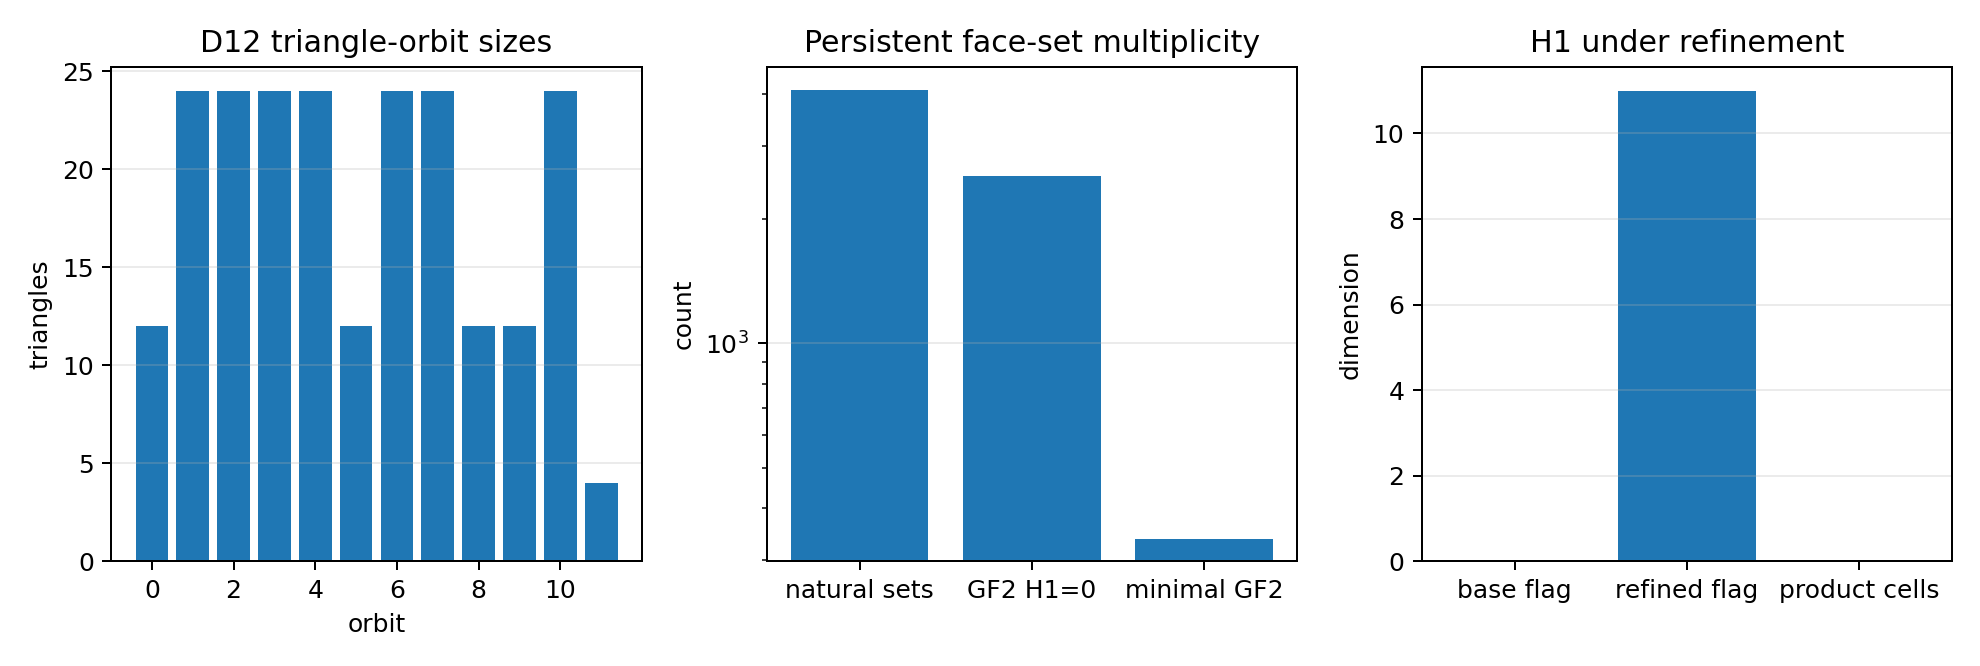
\includegraphics[width=.98\textwidth]{FIN_ST1902_ST1991_Figures/cell_complex_no_go_summary.png}
\caption{Left: the twelve triangle-orbit sizes.  Centre: face-set multiplicity
persists after topology/minimality gates.  Right: the flag complex acquires
eleven $H^1$ modes under refinement; product squares remove them.}
\end{figure}

\section{Most important result}

The most important conclusion is:
\[
\boxed{
\text{no canonical gauge curvature geometry follows from strict support and
basic naturality alone}.}
\]
This remains true after imposing vanishing first homology, minimal orbit
support, positive edge-derived measures, exact refinement and Hodge closure.

The constructive remnant is a \emph{relative} cellular category: after choosing
a base complex and retaining the explicit refinement morphism, lift base faces
and add product squares/cubes.  It is functorial relative to the history, but
its initial complex and Hodge weights remain unsourced.

\section{Highest-value next theorem}

The next problem with the greatest power to decide whether FIN can generate
gauge physics is:
\begin{quote}
\emph{Classify all positive face inner products for which gauge-curvature
energy commutes with FIN coarse/refinement maps over $12\to24\to48$, and prove
either uniqueness up to one overall scale or a nonuniqueness theorem.}
\end{quote}

Required tests are existence, positivity, automorphism naturality, the
$12\to24$ energy identity, $24\to48$ associativity, uniqueness modulo scale,
and controlled continuum scaling.  A failure would block strict gauge geometry
without new assumptions.  A unique solution would supply the first serious
candidate for a strict Hodge/Wilson action.

\section{Route ranking}

\begin{longtable}{@{}p{.53\textwidth}p{.18\textwidth}p{.18\textwidth}@{}}
\toprule
Route & Rigorous-success estimate & Physics decision power \\
\midrule\endhead
classify energy-preserving Hodge measures across $12$--$24$--$48$ & 0.42 & 1.00 \\
develop conditional product-cell $U(1)$ lattice model & 0.82 & 0.50 \\
support-only flag spectral action & 0.15 & 0.55 \\
continue APD/moment $L_{\rm total}$ repair & 0.01 & 0.35 \\
OA platform experiment & 0.45 & 0.55 \\
\bottomrule
\end{longtable}

These are strategic judgments, not empirical probabilities.

\section{Final interpretation}

\begin{quote}
FIN currently supports a clean conditional gauge-matter action and a relative
product-cell refinement, but not a unique strict gauge curvature geometry.
Automorphism symmetry, topology, flag naturality and spectral dimension do not
remove the choice of faces, Hodge weights or scaling.  FIN therefore remains a
finite Dirichlet--Markov--spectral information geometry with conditional gauge
extensions, not a fundamental physical theory.  The energy-preserving Hodge
classification is now the sharpest mathematical decision point.
\end{quote}

\appendix
\section{Six-round ledger}
\begin{longtable}{@{}p{.18\textwidth}p{.35\textwidth}p{.37\textwidth}@{}}
\toprule
Range & Target & Verdict \\
\midrule\endhead
ST1902--ST1916 & automorphism-natural faces & massive nonuniqueness \\
ST1917--ST1931 & face measures & positive natural cone nonunique \\
ST1932--ST1946 & refinement functor & flag/product conflict \\
ST1947--ST1961 & Wilson/continuum & positive conditional action, dimension free \\
ST1962--ST1976 & Hodge repair & support-only functor no-go \\
ST1977--ST1991 & synthesis & energy-compatible Hodge frontier \\
\bottomrule
\end{longtable}

\section{Reproducibility}
The authoritative result sets run from
\path{FIN_ST1902_ST1916_Results.json} through
\path{FIN_ST1977_ST1991_Results.json}.  Each contains fifteen programmes and
packet SHA-256 references.  The combined test
\path{test_fin_st1902_st1991.py} verifies all ninety packets, orbit counts,
exact ranks, measure rank, refinement homology, flag/Hodge obstruction, updated
gate, figure and nonpromotion boundaries.

\section{Nonclaims}
This report does not derive a base face set, Hodge measure, gauge coupling,
lattice spacing, continuum dimension, Lorentz signature, Maxwell normalization,
state ontology, apparatus or evidence.  It does not complete legacy role
transfer, QW-2191, Standard Model, gravity, $L_{\rm total}$ or Theory of
Everything.  All future FIN PDFs remain English.

\begin{thebibliography}{9}
\bibitem{hatcher} A. Hatcher, \emph{Algebraic Topology}, Cambridge University Press.
\bibitem{desbrun} M. Desbrun et al., Discrete Exterior Calculus, arXiv:math/0508341.
\bibitem{rothe} H. J. Rothe, \emph{Lattice Gauge Theories}, World Scientific.
\end{thebibliography}
\end{document}
